\documentclass[../thesis.tex]{subfiles}
\begin{document}

\chapter{validation}
\label{chp:validation}

Within this chapter the model validation is explained and described. At first the experimental setup used in the performed experiments is shown and then the experimental and model results are explained. After that a comparison is done to show that the model is performing as expected.

\section{experimental setup}

The experiments used for validating the developed model where done using a sounding rocket as part of the \texttt{MORABA} (\textbf{Mo}bile \textbf{Ra}cketen \textbf{Ba}sis) \cite{stamminger2012moraba} setup. The mission's name was \texttt{TEXUS-57}. The experimental setup as shown in \cite{stergiou2022effects} is visible in \autoref{fig: experiment}.
\begin{figure}[htbp]
	\centering
	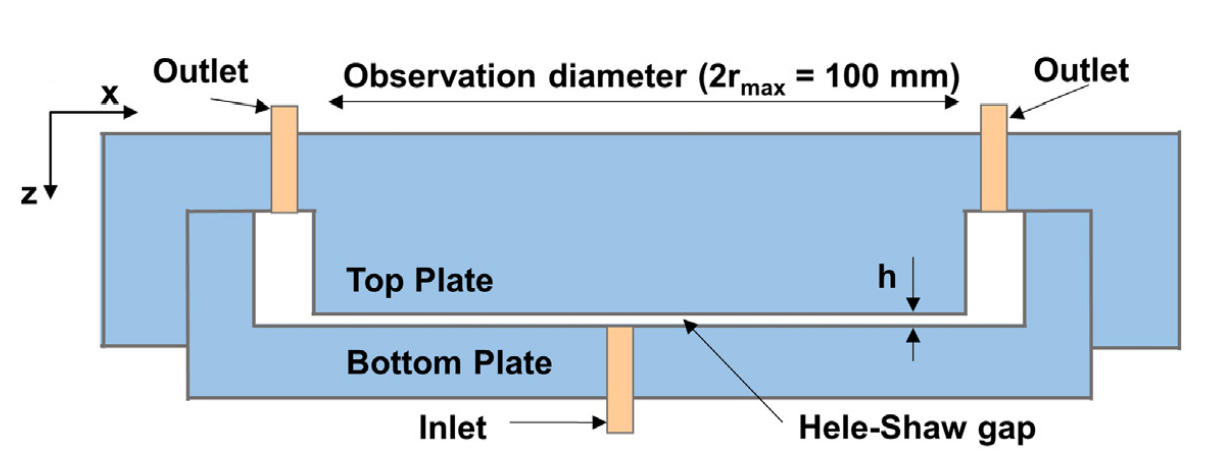
\includegraphics[scale=0.4]{experimental_setup}
	\caption{experimental setup for validation \cite{stergiou2022effects}}
	\label{fig: experiment}
\end{figure}
The gap height $h$ used for the experiments was 0.2 mm. The experiment is observed by a camera from the top throughout the hole run. These gained images are the base for further analysis.

\section{experimental results}

An image example as gained by the experiments is shown in \autoref{fig: exp_img}. The analysis on this images is done using image processing. The image is converted to a gray-scale image as a first step. Then the gained values are correlated to concentration values using the known values for the input's concentrations. Based on the gained product concentration values the reaction front's front and back positions are gained by a threshold operation. The position of the fronts maximum is computed by detecting the position of the maximum gray value within the image. The results are stored within \texttt{.csv} files. The file containing the fronts position has the form shown in \autoref{tab: front_csv}. 

\begin{table} [htb]
	\centering
	\caption{front position output format}
	\begin{tabular}{ cccc }
		\hline
		t (s) & WC (mm) & RC (mm) & Rf (mm) \\
		\hline
		46.333 & 2.4949 & 5.6819 & 8.1854 \\
		... & ... & ... & ... \\
		52 & 3.0455 & 6.2054 & 8.7207 \\
		... & ... & ... & ... \\
		\hline
		\label{tab: front_csv}
	\end{tabular}
\end{table}
t describes the flow time during the experiment in seconds and WC is front's width. The width is calculated using the difference between the front's front and back positions. RC is the radial distance from the center of the front's maximum and Rf is the front's front position.
In addition to the front's positions the total amount of product formed is calculated. This is done by integrating the concentration values over the hole domain and gap height. To make experiments more easily comparable with each other the formed product values (in mol) are non-dimensionalized. To achieve this the values are divided by $c_{max} \cdot V_{reactor}$. The variable $c_{max}$ is the maximum value of the product's concentration during one experimental run and $V_{reactor}$ is the reactor's volume. The product of these two values refers to the fully mixed case as it gives in indication of the maximum amount of product possible than can be created. The format of the results is shown in \autoref{tab: product_csv}. The volume injected is equivalent to the time elapsed in seconds. These two values can be converted using the flow rate. NC is the non-dimensional product formed for each time step.

\begin{table} [htb]
	\centering
	\caption{product formed output format}
	\begin{tabular}{ cc }
		\hline
		Volume injected (mL) & NC (-) \\
		\hline
		0 & 0.011312 \\
		... & ... \\
		0.01072 & 0.011907 \\
		... & ... \\
		\hline
		\label{tab: product_csv}
	\end{tabular}
\end{table}

\section{model results}
\label{sec: model res}

The results gained from the model are no images but tables with all exported values. These tables are created at each interval defined by the user as described in \autoref{sec: setup}. The tables do have a format similar to \autoref{tab: model_csv}. The values for each cell are stored in one of the tables rows. The cells are distinguishable by their x and y coordinate.

\begin{table} [htb]
	\centering
	\caption{simulation output table example}
	\small
	\begin{tabular}{ cccccc }
		\hline
		nodenumber & x-coordinate & y-coordinate & ... & concentration-fluid\_c & ... \\
		\hline
		1 & 1.206592076E-06 & 5.0E-04 & ... & 5.681614735E-11 & ...\\
		... & ... & ... & ... & ... & ... \\
		100 & 1.382432295E-06 & 5.12E-04 & ... & 3.607185187E-17 & ... \\
		... & ... & ... & ... & ... & ... \\
		\hline
		\label{tab: model_csv}
	\end{tabular}
\end{table}

All values needed are accessible with these tables but for further analysis the values need to be converted into a field similar two the created mesh during model setup. An example of such a resulting field is shown in \autoref{fig: field_example}.
\begin{figure}[htbp]
	\centering
	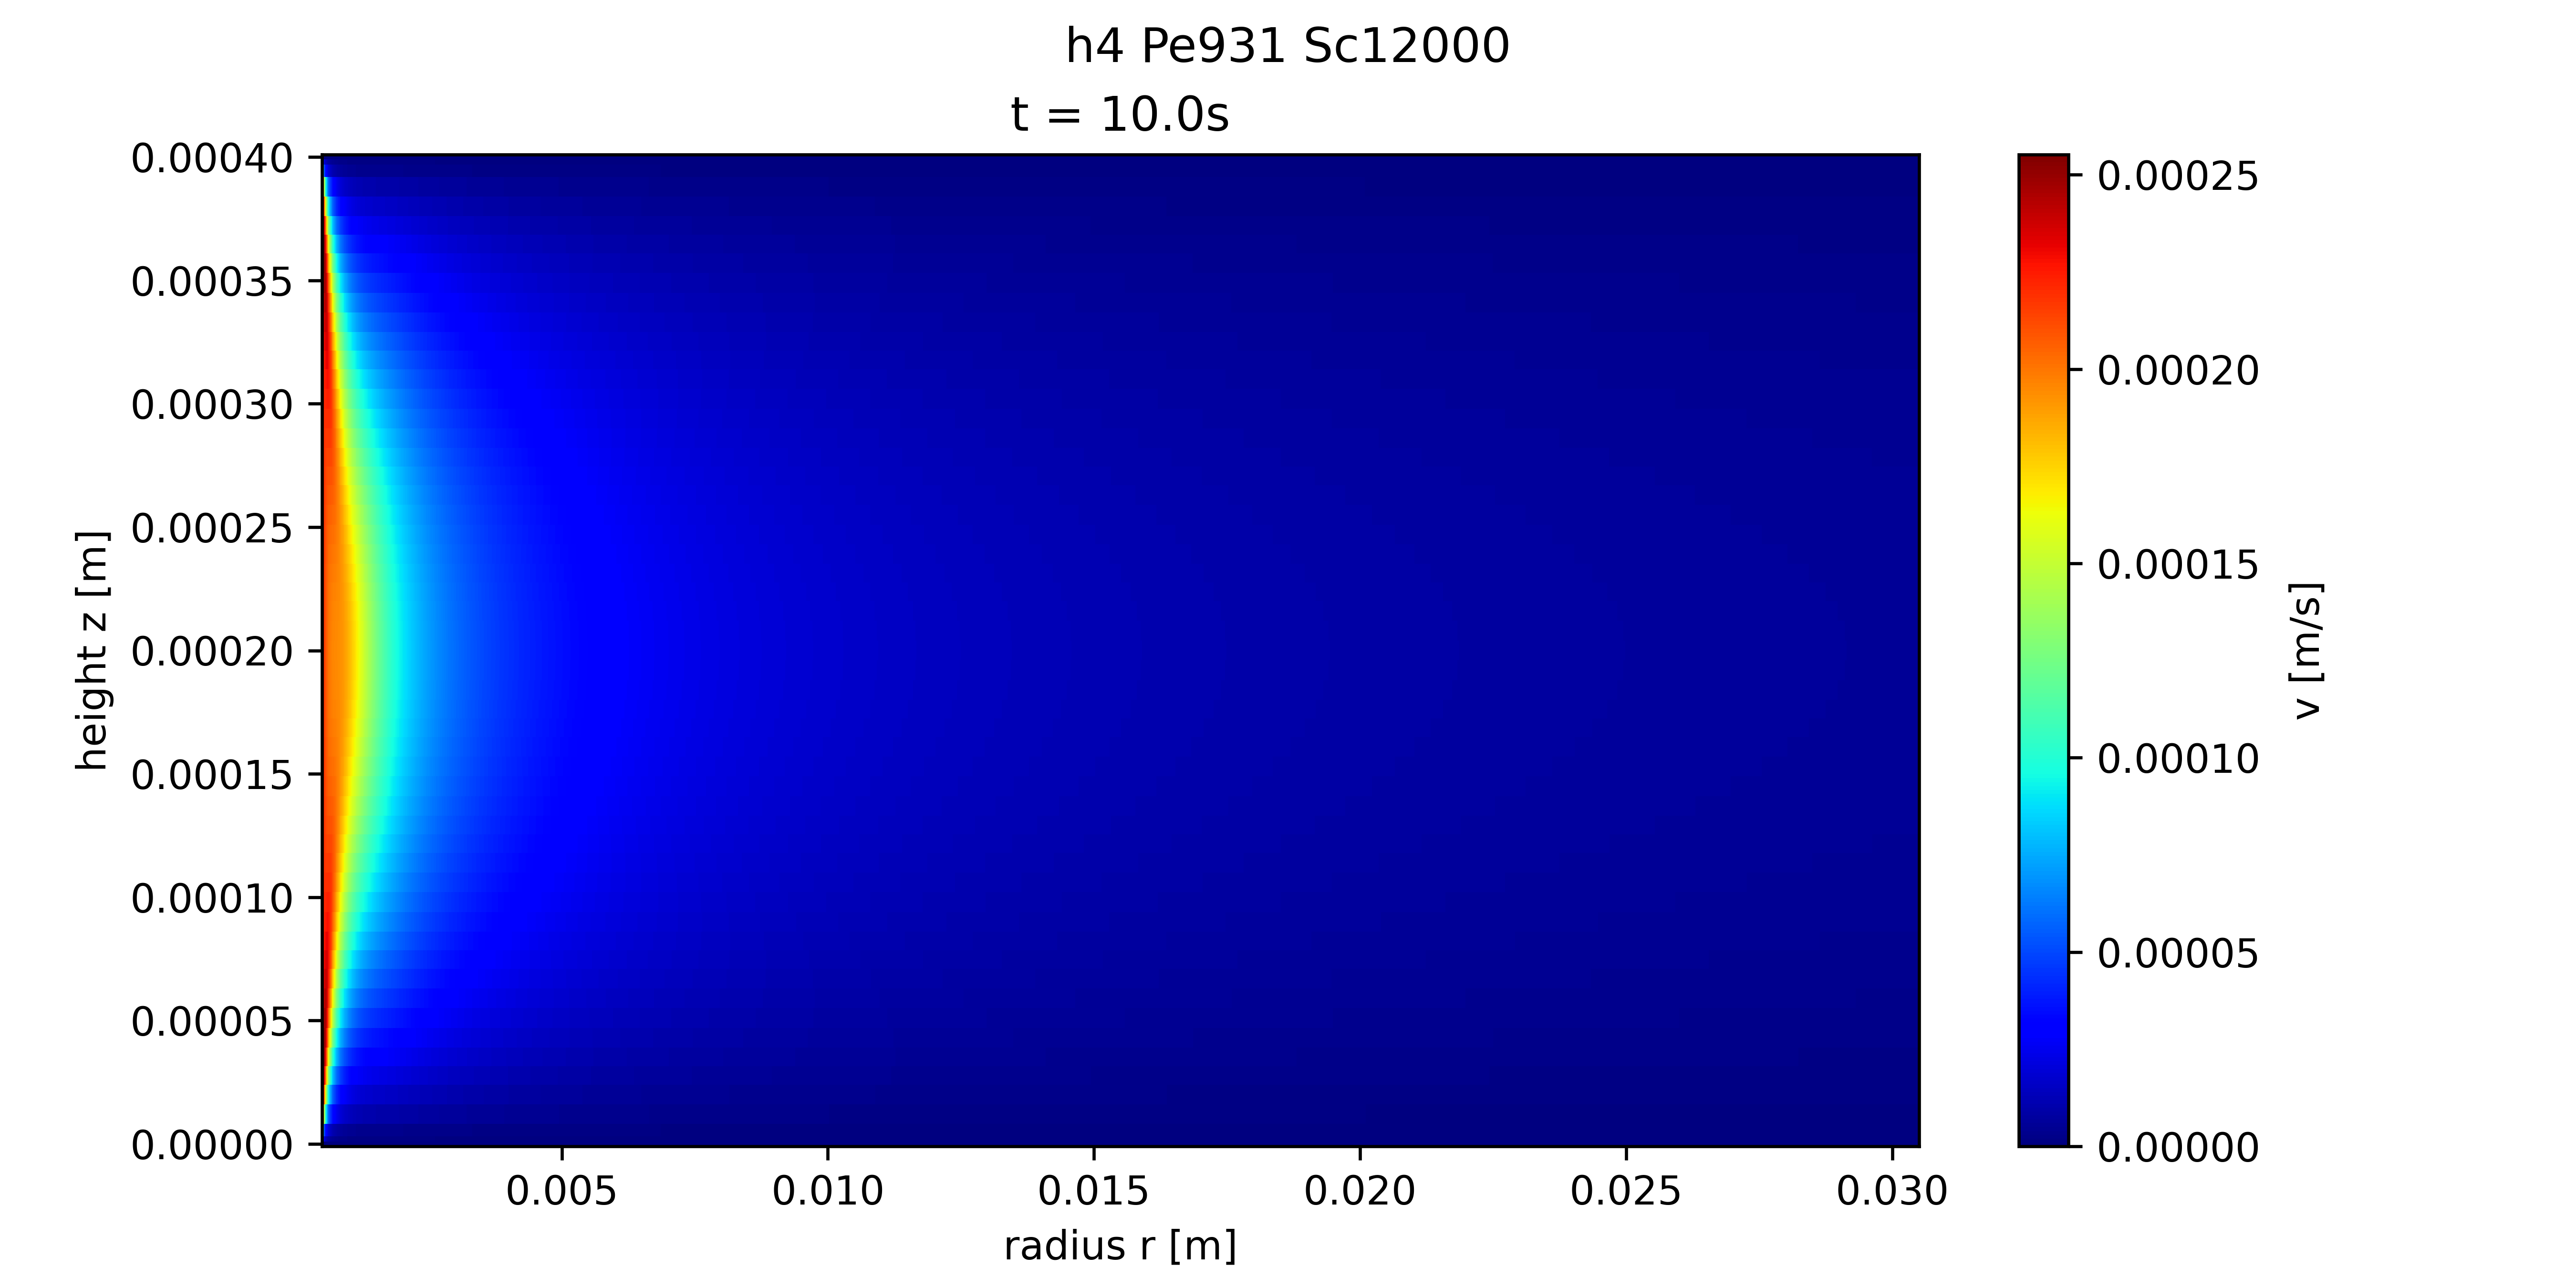
\includegraphics[width=\textwidth]{field_example}
	\caption{example field representation of model results}
	\label{fig: field_example}
\end{figure}
These can be created for all exported variables. Within the example shown the field is created for the velocity magnitude but the variable of most interest is the product concentration. A field example for this variable is shown in \autoref{fig: c_prod_examp} for 3 different time steps.
\begin{figure}[htbp]
	\centering
	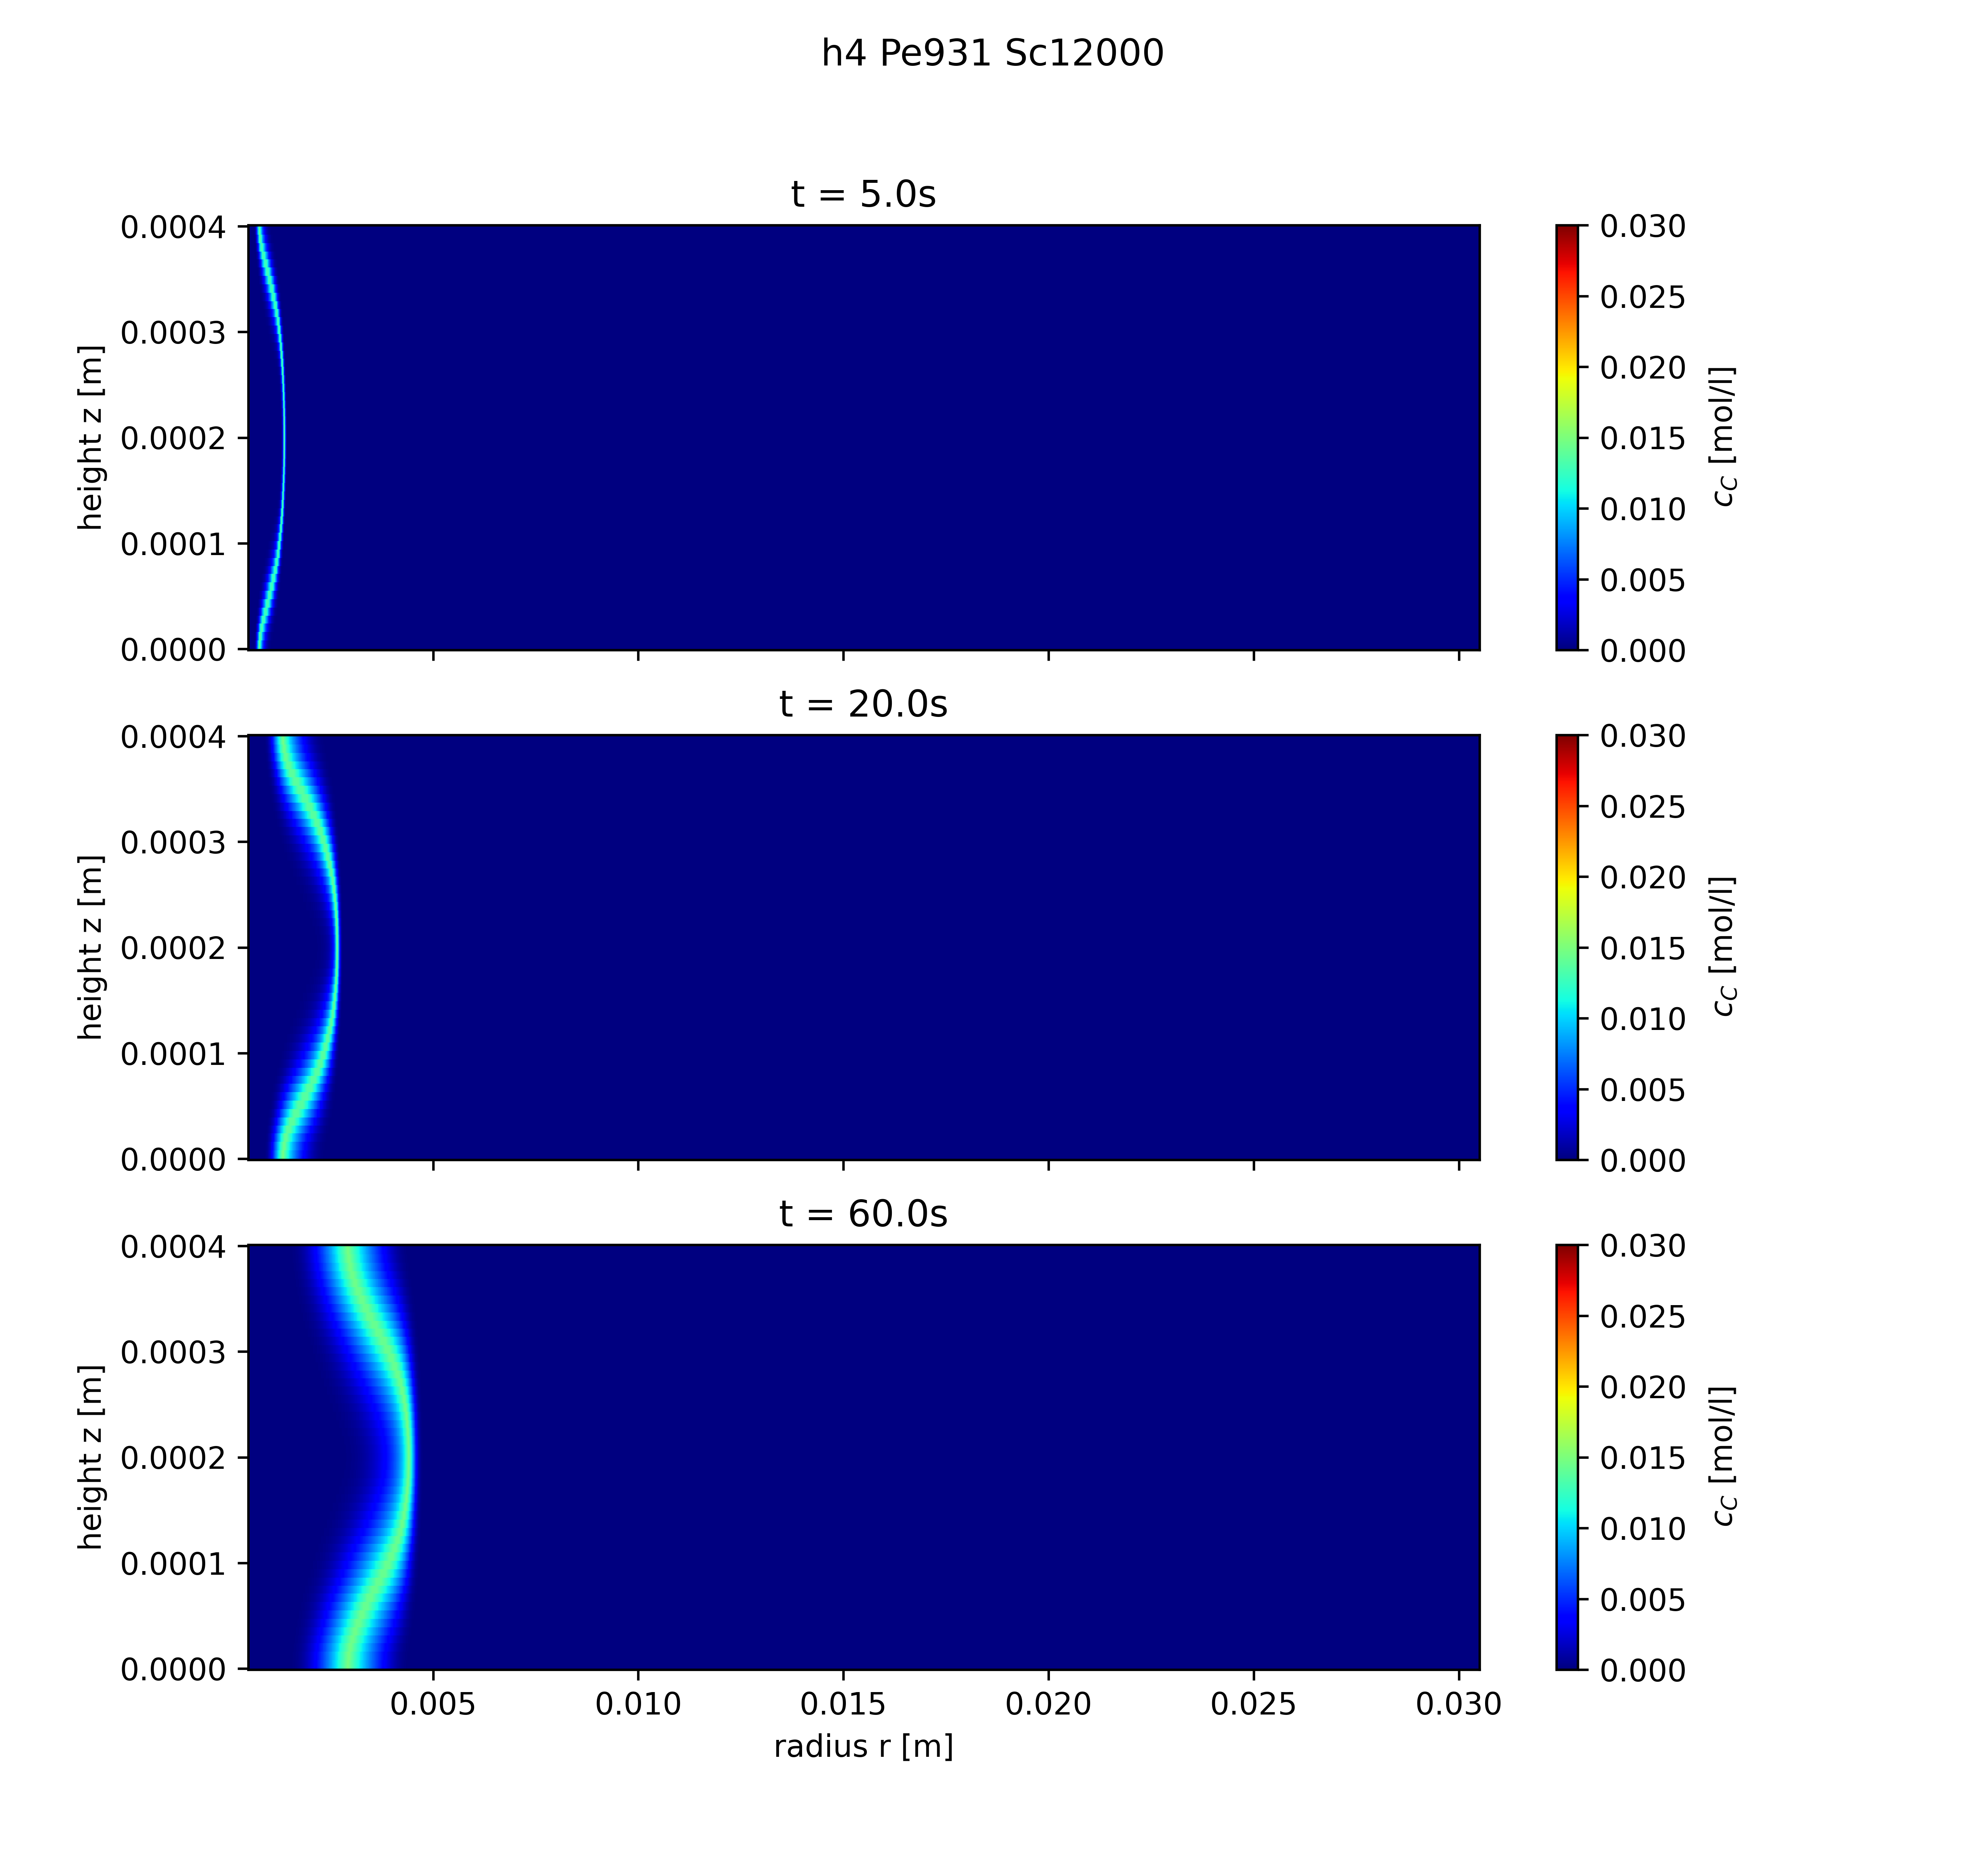
\includegraphics[width=\textwidth]{c_prod_example}
	\caption{example product concentration fields}
	\label{fig: c_prod_examp}
\end{figure}
With these fields the product's concentration can be averaged over the hole gap height. This step is done to get a comparable post-processing step to the image processing done on the experimental data sets. The resulting plots from the previous example can be seen in \autoref{fig: c_plot_examp}.
\begin{figure}[htbp]
	\centering
	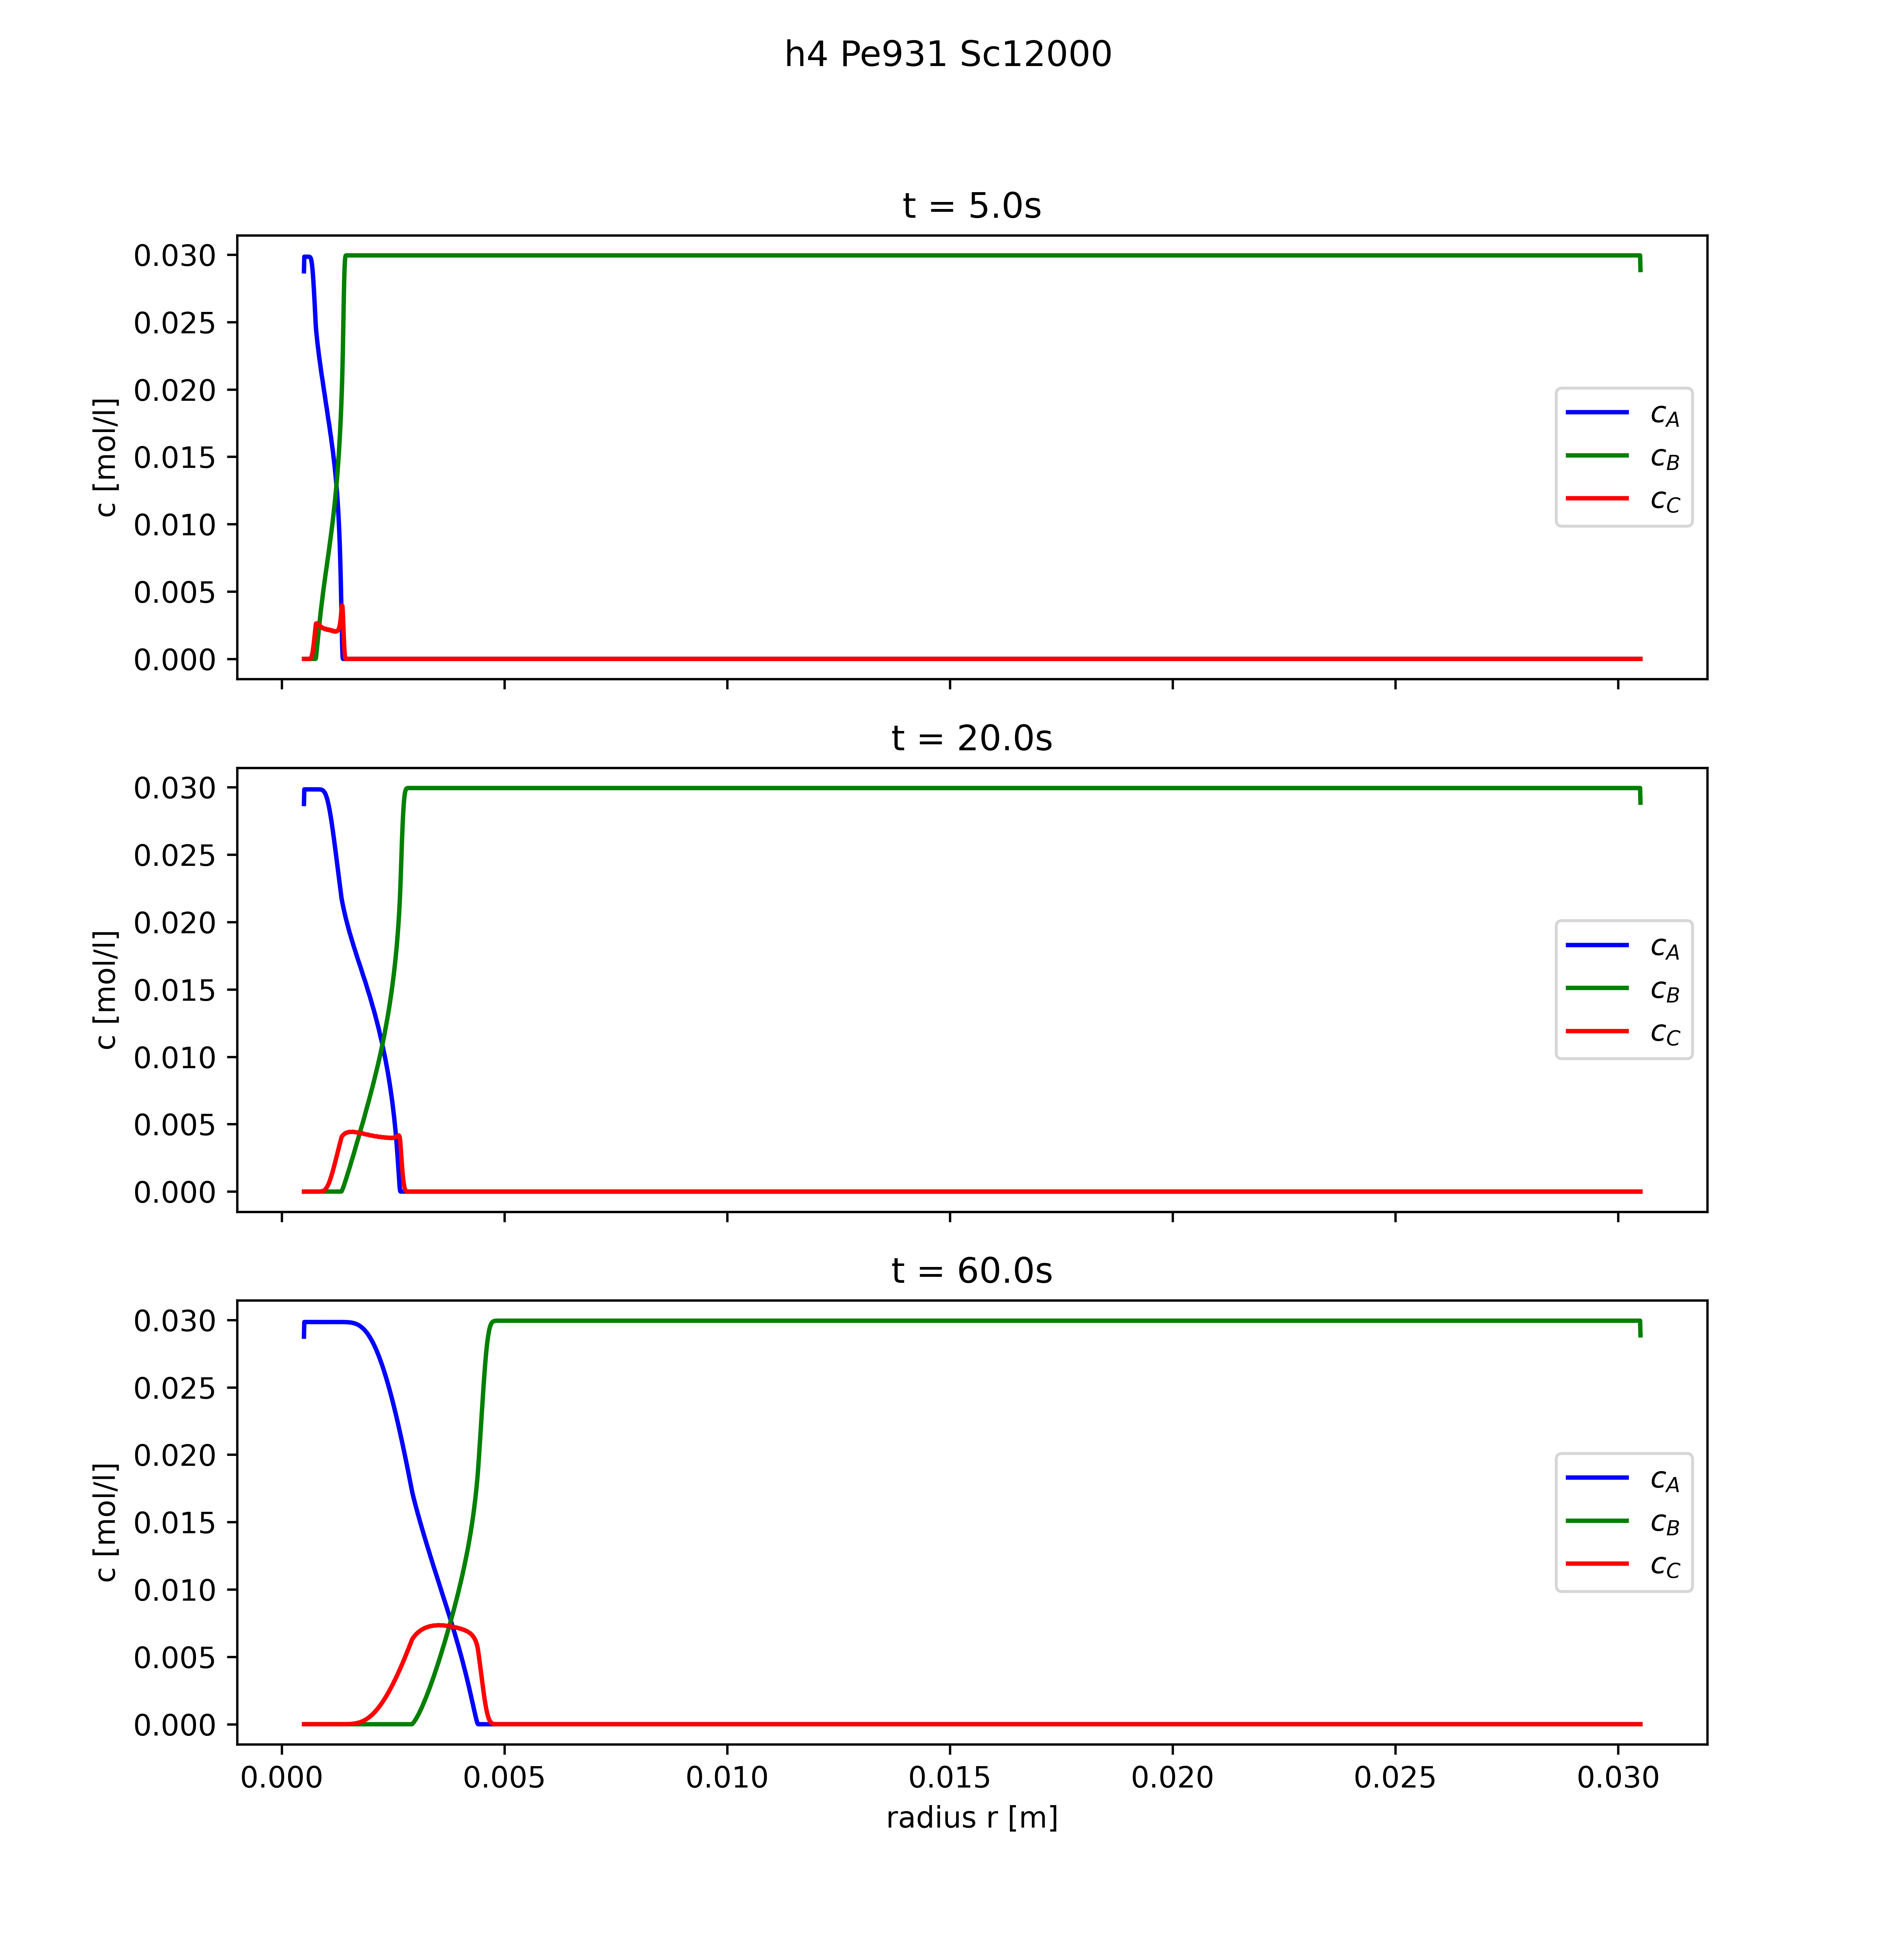
\includegraphics[width=\textwidth]{c_plot_example}
	\caption{example gap averaged product concentration plots}
	\label{fig: c_plot_examp}
\end{figure}

With the fields and the gap averaged concentration values computed the parameters of interest can be calculated which is explained within the following sections.

\subsection{front positions}

The front's maximum position is gained by storing the radial positions of the product's maxima within the concentration plots. The front's front position is calculated by using the the position furthest away from the center at half the maximums value. The positions gained are shown for one time step in \autoref{fig: pos_examp} as an example.

\begin{figure}[htb]
	\centering
	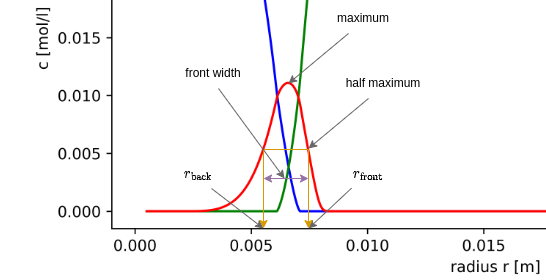
\includegraphics[scale=0.5]{positions_examp}
	\caption{front position procedure schematic}
	\label{fig: pos_examp}
\end{figure}

\subsection{front width}

For calculating the front widths the fronts front and back positions are needed. The front position is already gained and the back position is computed using the same approach. Instead of taking for furthest position away from the center the closest one to the inlet is taken to get the back position. The difference between these two radial positions is the front's width at the time. The width calculated is visualized in \autoref{fig: pos_examp}.

To gain some more insights a second width is computed. The second width is calculated at the middle of the gap using the same procedure. Instead of taking the gap averaged values, the values used here are the field values themselves at half the gap height.

\subsection{product formed}

Since the cell volume and the product concentration for each cell are exported the total amount of product formed can be calculated ba multiplying these two columns with each other. \texttt{ANSYS FLUENT} computes it's values for one radiant for a 2D case. To gain the amount of product within the hole reactor the values have to be multiplied by $2 \pi$. This procedure can be described by \autoref{eqn: tot_prod}. $ n_{C, total} $ is the total amount of product produced, $n_{cells}$ is the amount of cells in the mesh, $ V_i $ is the volume of one cell and $c_{i, C}$ the product's concentration within that cell $i$.

\begin{equation}
	n_{C, total} = 2 \pi \cdot \sum_{i=0}^{n_{cells}} \left[ V_i \cdot c_{i, C} \right]
	\label{eqn: tot_prod} 
\end{equation}

\section{comparison}

For comparison the position of the product's maximum is used. It can be seen that the model and experiment perform similar over hole time range with a small deviation at the early time steps. These difference might come from slightly different flow condition or some mixing due to gravitational influence. Further reasons and possible explanations for the differences within model and experimental results are discussed within \autoref{chp:err_lims}.

\begin{figure}[htbp]
	\centering
	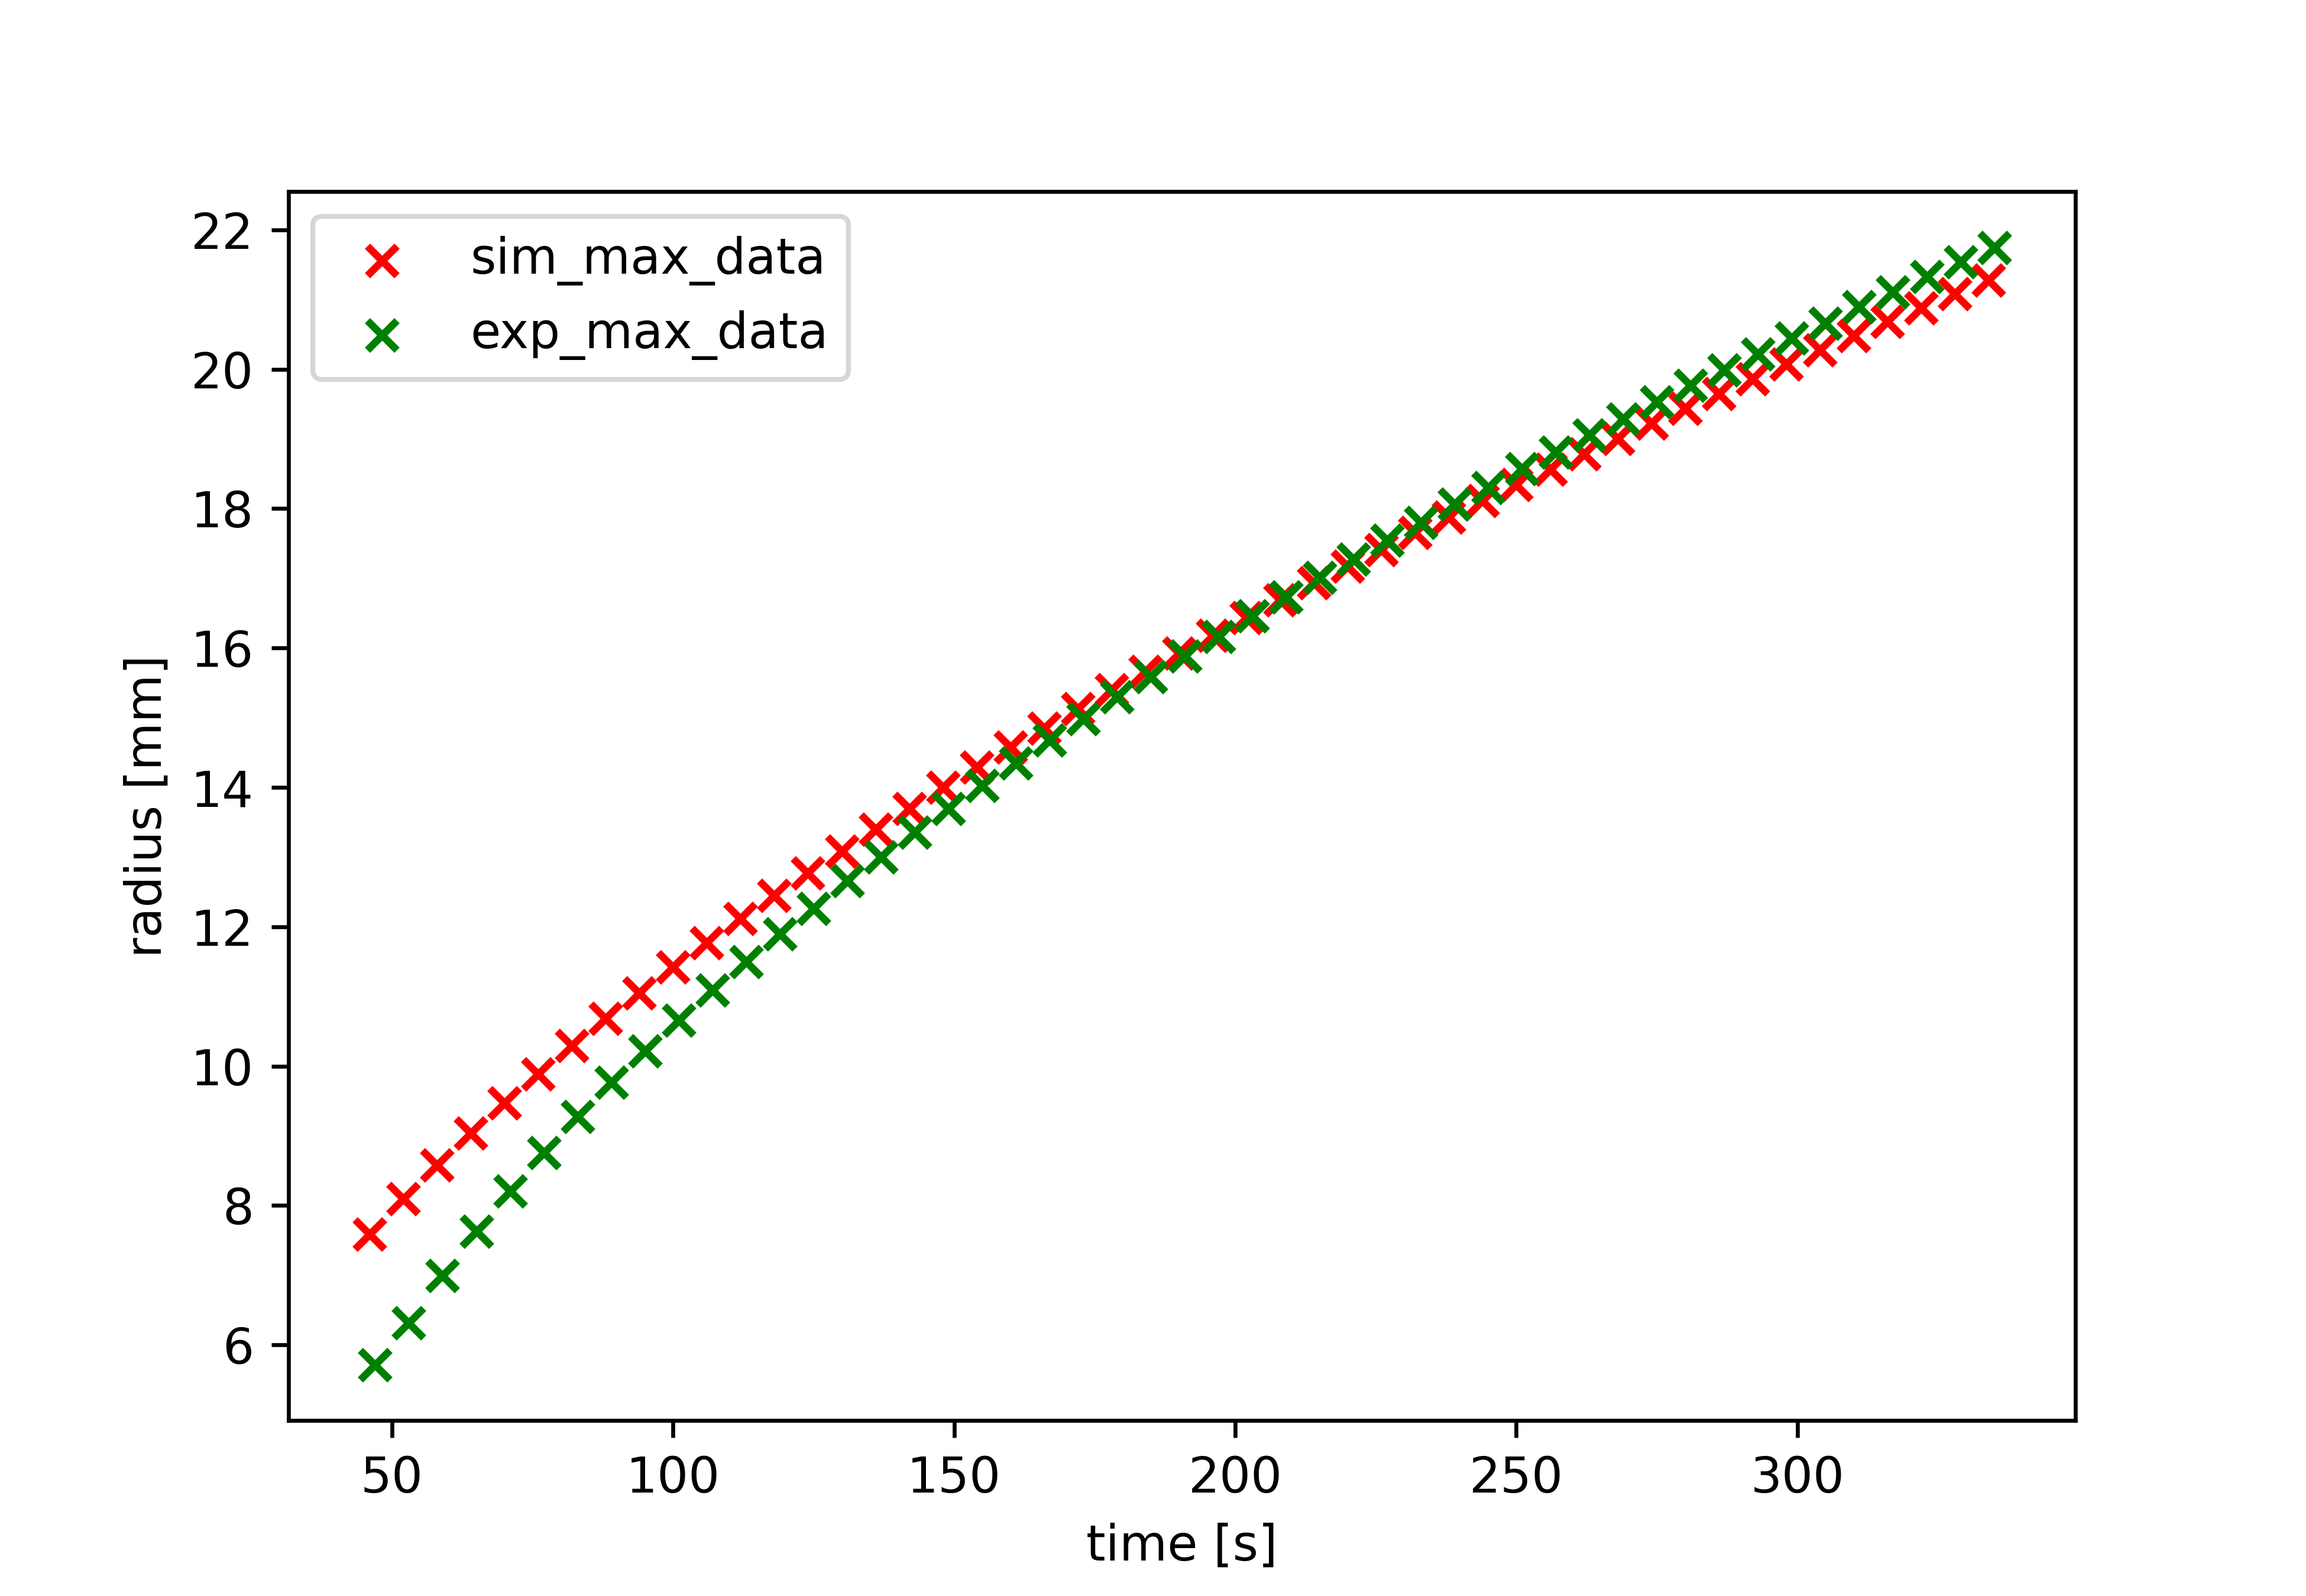
\includegraphics[width=\textwidth]{front_exp}
	\caption{comparison of the experimental and model maxima positions}
	\label{fig: comp_maxis}
\end{figure}

\end{document}